\documentclass[journal]{IEEEtran}
\usepackage[a5paper, margin=10mm, onecolumn]{geometry}
\usepackage[cmex10]{amsmath}
\usepackage{amssymb,amsfonts,amsthm}
\usepackage{gvv-book}
\usepackage{gvv}
\usepackage{hyperref}

\begin{document}

\title{1.5.33}
\author{Puni Aditya - EE25BTECH11046}
\maketitle

\textbf{Question:}\\
Find the ratio in which the Y-axis divides the line segment joining the points A\brak{5, -6} and B\brak{-1, -4}. Also find the coordinates of the point of intersection.

\textbf{Solution:}\\
Let the given points be A and B
\begin{align*} \vec{A} = \myvec{5 \\ -6}, \vec{B} = \myvec{-1 \\ -4} \end{align*}
Let the Y-axis divide the line segment $\vec{AB}$ at point $\vec{P}$ in the ratio $k:1$.
Since $\vec{P}$ lies on Y-axis, let
\begin{align*}
\vec{P} = \myvec{0 \\ y}
\end{align*}
The point $\vec{A}$, $\vec{B}$, $\vec{P}$ are collinear.
\begin{align}
\implies \text{rank}\myvec{\vec{B}-\vec{A} & \vec{P}-\vec{A}} = 1
\end{align}
\begin{align}
\myvec{-6 & -5 \\ 2 & y+6} \xleftrightarrow[]{R_2 \rightarrow {\frac{1}{3}R_1 + R_2}}\myvec{-6 & -5 \\ 0 & y+\frac{13}{3}}  
\end{align}
The number of nonzero rows in the row reduced matrix (also known as {\em echelon form}) is defined as the rank. For above matrix to be of rank 1,
\begin{align}
y+\frac{13}{3} &= 0 \\
y &= \frac{-13}{3}
\end{align}
$\therefore$ The coordinates of the point of intersection are 
\begin{align*}
\vec{P} = \myvec{0 \\ \frac{-13}{3}}
\end{align*}

Substituting the values of $\vec{A}$, $\vec{B}$ and $\vec{P}$,
\begin{align}
k=\frac{\myvec{5 & \frac{-5}{3}}\myvec{1 \\ \frac{-1}{3}}}{\norm{\myvec{1 \\ \frac{-1}{3}}}^2}=5
\end{align}

Thus, the ratio in which the point $\vec{P}$ divides the line segment $\vec{AB}$ is \textbf{5:1}. \\

\begin{figure}
    \centering
    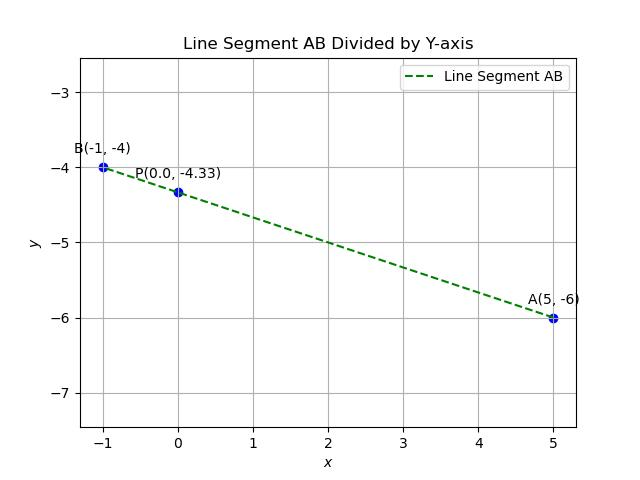
\includegraphics[width=0.5\columnwidth]{figs/plot_c.jpg}
    \caption*{Plot of Intersection of AB by Y-axis}
    \label{fig:fig}
\end{figure}

\end{document}
